\subsection{Traditional cuts on the proton lab coordinates $\phi, \theta, p$}
The fiducial cut in the lab coordinates has been determined during the $\pi^0$ analysis in
the $\Delta(1232)$ region \cite{bib:pi0_Delta}.
For each momentum and theta bin the $\phi$ distributions were fitted with the trapezoid function shown in appendix ~\ref{sec:p_tent_function}.
The resulting parameters were fitted as a function of the $\theta$ with a fourth order polynomial.
Fig.~\ref{fig:traped_fit_result_s5} shows the calculated $\phi_{MIN}$ and $\phi_{MAX}$  and the resulting fit
for sector 5 and momentum range $0.9$ to $1.6$ GeV.

\begin{figure}[h]
    \begin{center}
        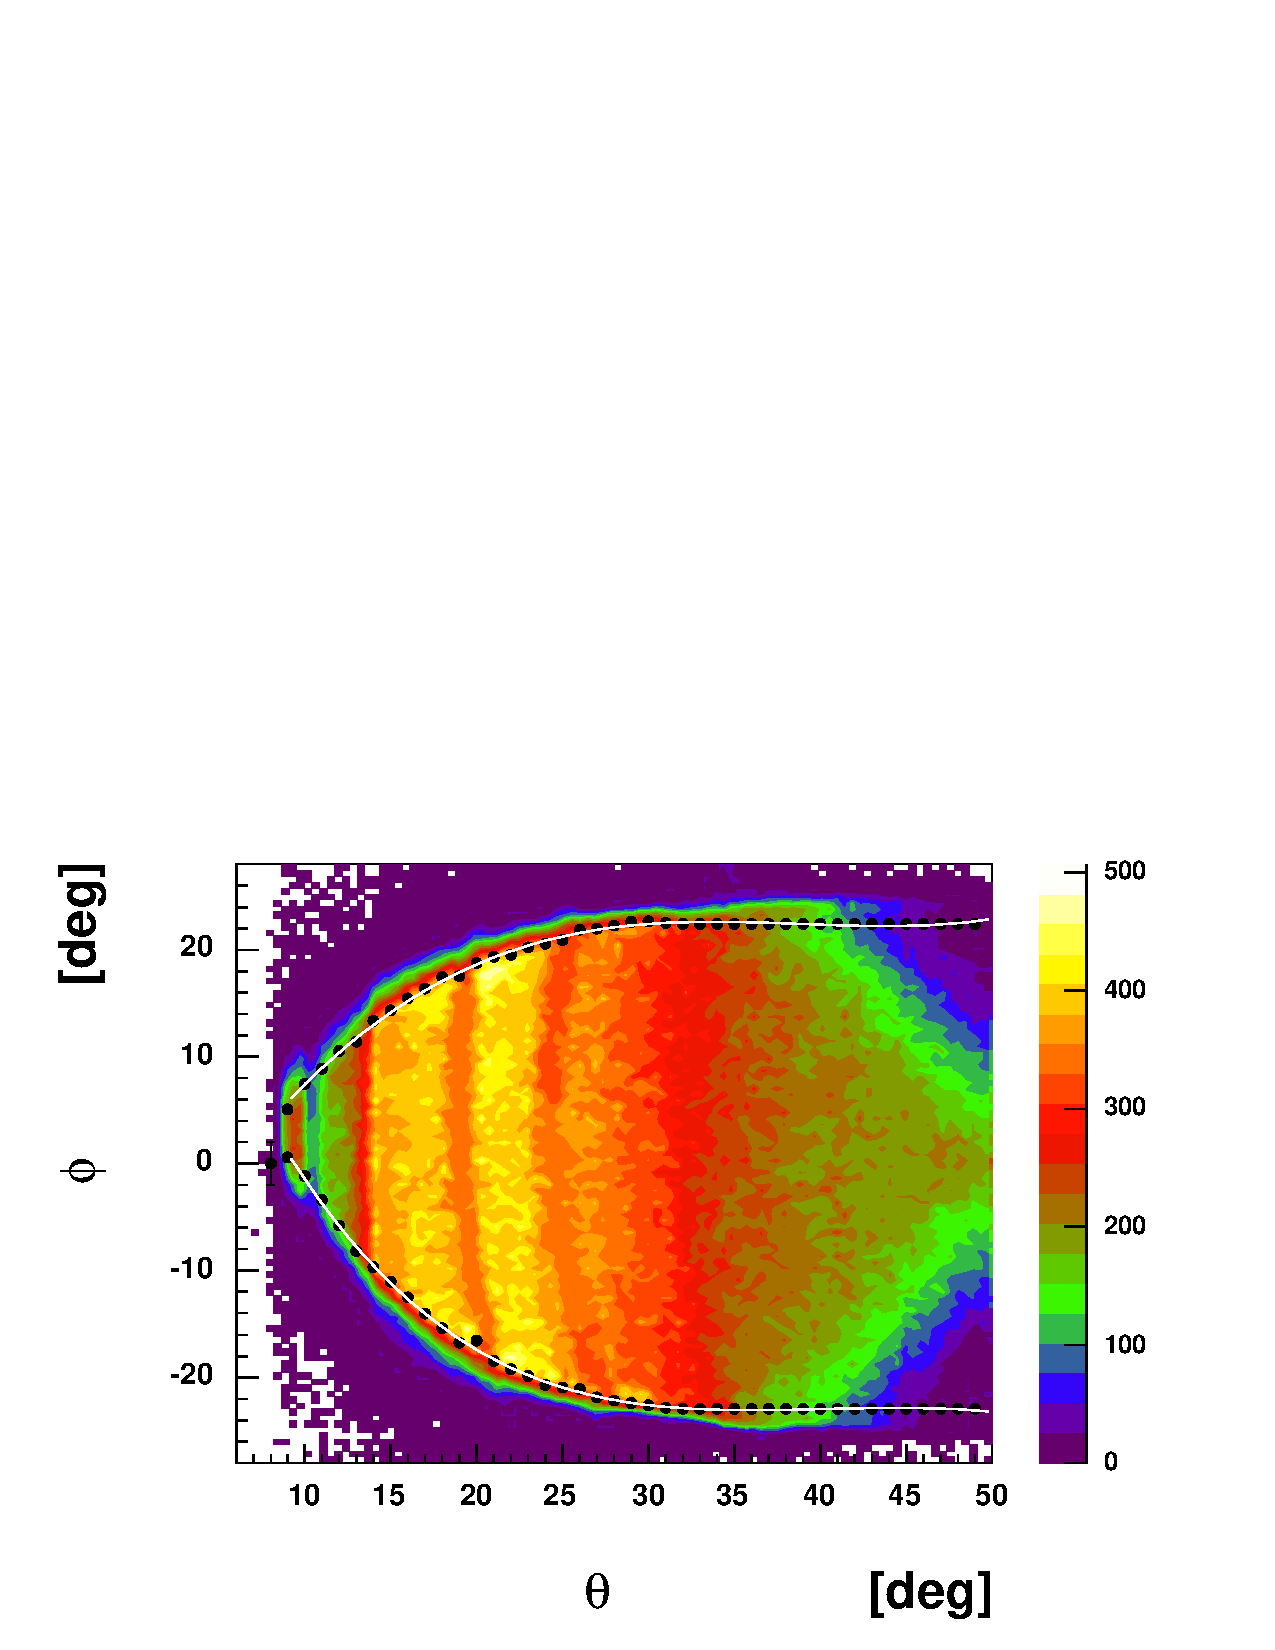
\includegraphics[width = 13cm, bb=0 0 580 430]{img/traped_fit_result_s5}
        \caption[Result of the trapezoid fit]
        { Result of the trapezoid fit for sector 5. The proton momentum ranges from $0.9$ to $1.6$ GeV.
        The black points are the parameters $p_1$ (negative $\phi$) and $p_2$ (positive $\phi$)
            for each $\theta$ slice fit.
        The white line is a fourth order polynomial fit to the black points.
        Unlike the electron case, the $\phi$ boundaries are asymmetric}
        \label{fig:traped_fit_result_s5}
    \end{center}
\end{figure}

\subsection{ $\theta$ versus momentum cuts}
Sector 2, 3, 5 and 6 present holes and depletions which were taken care of with the
cuts shown on Fig.~\ref{fig:proton_tp} where $\theta$ is plotted against the momentum $p$.

\begin{figure}[h]
    \begin{center}
        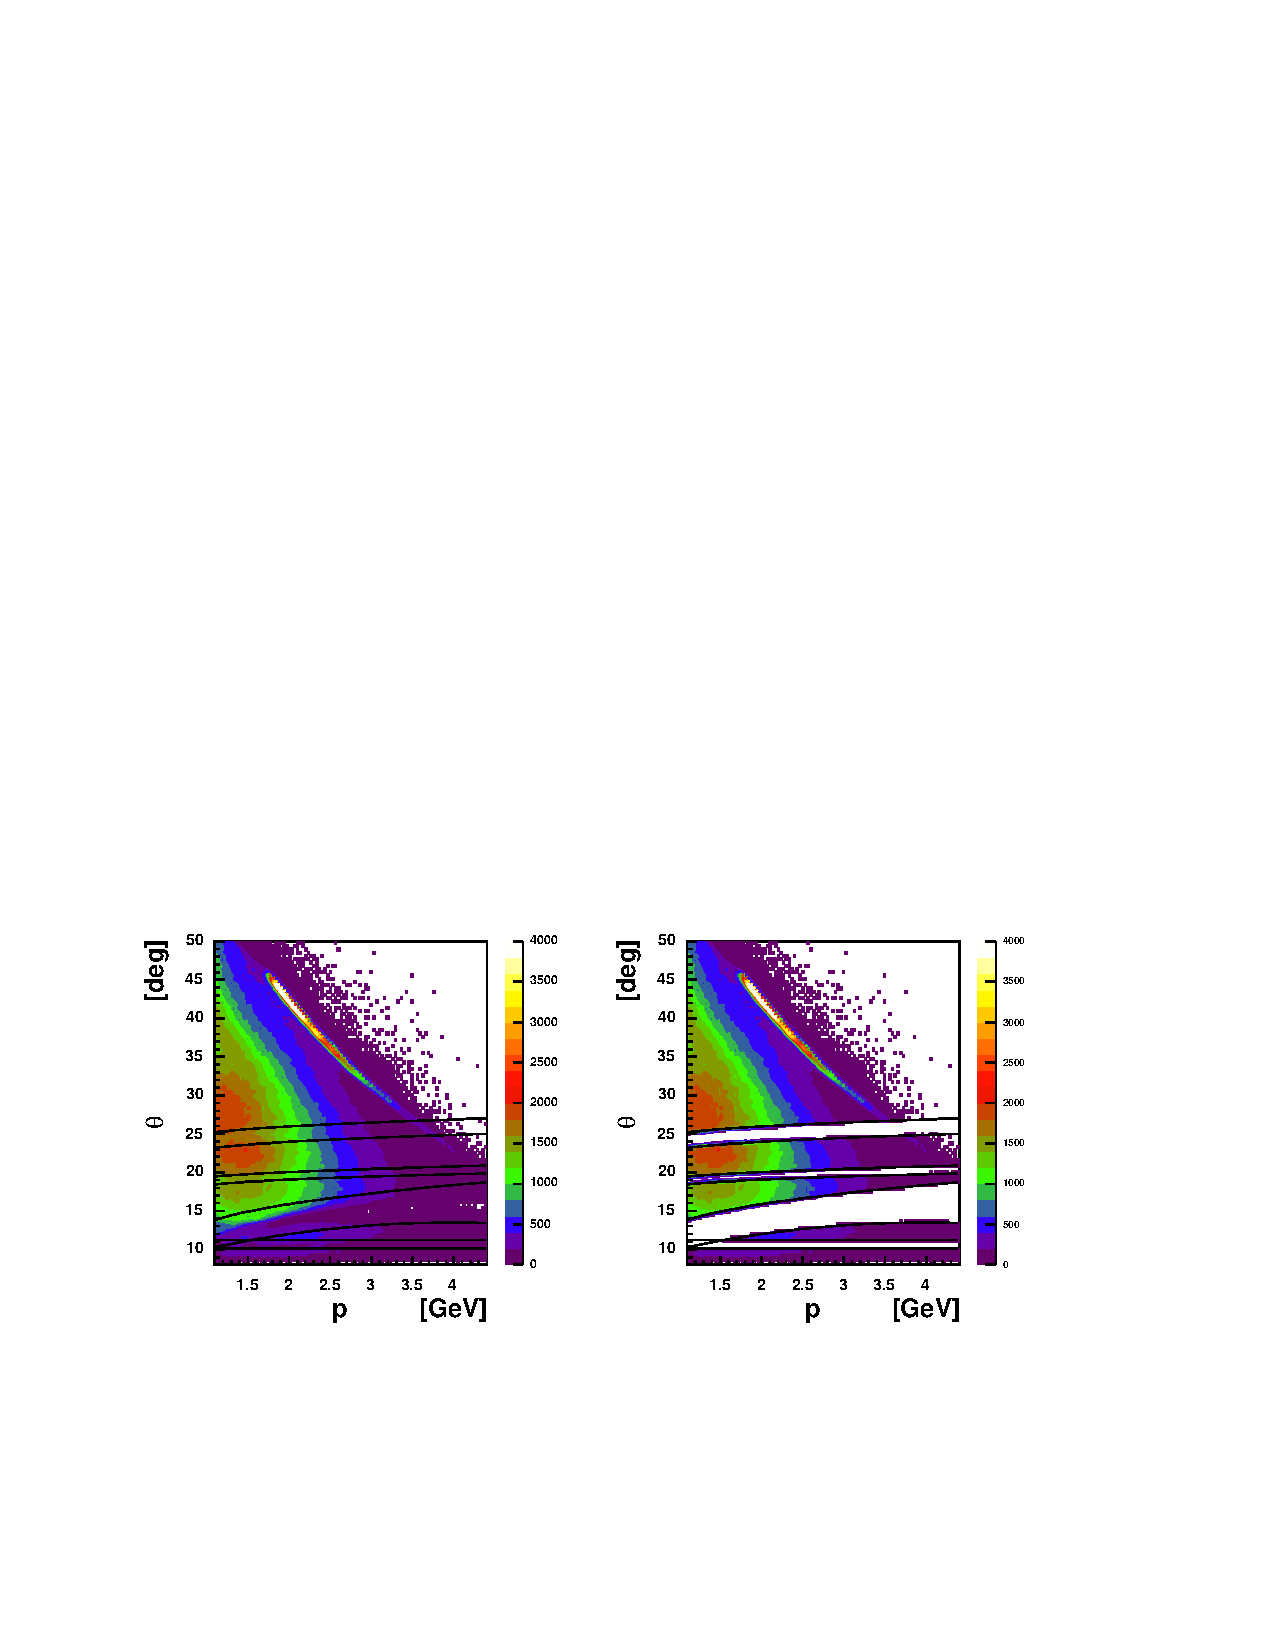
\includegraphics[width=0.98\textwidth]{img/proton_tp}
        \caption[$\theta$ versus $p$ for protons sector 5]
        { $\theta$ versus $p$ for protons sector 5. A depletion is clearly visible and cut out.}
        \label{fig:proton_tp}
    \end{center}
\end{figure}




